\documentclass{book}
% psfigTeX macros
%
% All software, documentation, and related files in this distribution of
% psfig/tex are Copyright (c) 1987 Trevor J. Darrell
%
% Permission is granted for use and non-profit distribution of psfig/tex 
% providing that this notice be clearly maintained, but the right to
% distribute any portion of psfig/tex for profit or as part of any commercial
% product is specifically reserved for the author.
%
% Psfig/TeX Release 1.2
%
% file last modified: $Header: psfig.tex,v 1.3 88/11/22 01:23:34 van Exp $
%
\catcode`\@=11\relax
\newwrite\@unused
\def\typeout#1{{\let\protect\string\immediate\write\@unused{#1}}}
\typeout{psfig/tex 1.2}
%
% @psdo control structure -- similar to Latex @for.
% I redefined these with different names so that psfig can
% be used with TeX as well as LaTeX, and so that it will not 
% be vunerable to future changes in LaTeX's internal
% control structure,
%
\def\@nnil{\@nil}
\def\@empty{}
\def\@psdonoop#1\@@#2#3{}
\def\@psdo#1:=#2\do#3{\edef\@psdotmp{#2}\ifx\@psdotmp\@empty \else
    \expandafter\@psdoloop#2,\@nil,\@nil\@@#1{#3}\fi}
\def\@psdoloop#1,#2,#3\@@#4#5{\def#4{#1}\ifx #4\@nnil \else
       #5\def#4{#2}\ifx #4\@nnil \else#5\@ipsdoloop #3\@@#4{#5}\fi\fi}
\def\@ipsdoloop#1,#2\@@#3#4{\def#3{#1}\ifx #3\@nnil 
       \let\@nextwhile=\@psdonoop \else
      #4\relax\let\@nextwhile=\@ipsdoloop\fi\@nextwhile#2\@@#3{#4}}
\def\@tpsdo#1:=#2\do#3{\xdef\@psdotmp{#2}\ifx\@psdotmp\@empty \else
    \@tpsdoloop#2\@nil\@nil\@@#1{#3}\fi}
\def\@tpsdoloop#1#2\@@#3#4{\def#3{#1}\ifx #3\@nnil 
       \let\@nextwhile=\@psdonoop \else
      #4\relax\let\@nextwhile=\@tpsdoloop\fi\@nextwhile#2\@@#3{#4}}
% 
%
\def\psdraft{
	\def\@psdraft{0}
	%\typeout{draft level now is \@psdraft \space . }
}
\def\psfull{
	\def\@psdraft{100}
	%\typeout{draft level now is \@psdraft \space . }
}
\psfull
\newif\if@prologfile
\newif\if@postlogfile
\newif\if@noisy
\def\pssilent{
      \@noisyfalse
}
\def\psnoisy{
      \@noisytrue
}
\psnoisy
%%% These are for the option list.
%%% A specification of the form a = b maps to calling \@p@@sa{b}
\newif\if@bbllx
\newif\if@bblly
\newif\if@bburx
\newif\if@bbury
\newif\if@height
\newif\if@width
\newif\if@rheight
\newif\if@rwidth
\newif\if@clip
\newif\if@verbose
\def\@p@@sclip#1{\@cliptrue}
\def\@p@@sfile#1{%\typeout{file is #1}
		   \def\@p@sfile{#1}
}
\def\@p@@sfigure#1{\def\@p@sfile{#1}}
\def\@p@@sbbllx#1{
		%\typeout{bbllx is #1}
		\@bbllxtrue
		\dimen100=#1
		\edef\@p@sbbllx{\number\dimen100}
}
\def\@p@@sbblly#1{
		%\typeout{bblly is #1}
		\@bbllytrue
		\dimen100=#1
		\edef\@p@sbblly{\number\dimen100}
}
\def\@p@@sbburx#1{
		%\typeout{bburx is #1}
		\@bburxtrue
		\dimen100=#1
		\edef\@p@sbburx{\number\dimen100}
}
\def\@p@@sbbury#1{
		%\typeout{bbury is #1}
		\@bburytrue
		\dimen100=#1
		\edef\@p@sbbury{\number\dimen100}
}
\def\@p@@sheight#1{
		\@heighttrue
		\dimen100=#1
   		\edef\@p@sheight{\number\dimen100}
		%\typeout{Height is \@p@sheight}
}
\def\@p@@swidth#1{
		%\typeout{Width is #1}
		\@widthtrue
		\dimen100=#1
		\edef\@p@swidth{\number\dimen100}
}
\def\@p@@srheight#1{
		%\typeout{Reserved height is #1}
		\@rheighttrue
		\dimen100=#1
		\edef\@p@srheight{\number\dimen100}
}
\def\@p@@srwidth#1{
		%\typeout{Reserved width is #1}
		\@rwidthtrue
		\dimen100=#1
		\edef\@p@srwidth{\number\dimen100}
}
\def\@p@@ssilent#1{
	      \@verbosefalse
}
\def\@p@@sprolog#1{\@prologfiletrue\def\@prologfileval{#1}}
\def\@p@@spostlog#1{\@postlogfiletrue\def\@postlogfileval{#1}}
\def\@cs@name#1{\csname #1\endcsname}
\def\@setparms#1=#2,{\@cs@name{@p@@s#1}{#2}}
%
% initialize the defaults (size the size of the figure)
%
\def\ps@init@parms{
		\@bbllxfalse \@bbllyfalse
		\@bburxfalse \@bburyfalse
		\@heightfalse \@widthfalse
		\@rheightfalse \@rwidthfalse
		\def\@p@sbbllx{}\def\@p@sbblly{}
		\def\@p@sbburx{}\def\@p@sbbury{}
		\def\@p@sheight{}\def\@p@swidth{}
		\def\@p@srheight{}\def\@p@srwidth{}
		\def\@p@sfile{}
		\def\@p@scost{10}
		\def\@sc{}
		\@prologfilefalse
		\@postlogfilefalse
		\@clipfalse
		\if@noisy{
			\@verbosetrue
		}\else{
			\@verbosefalse
		}\fi
}
%
% Go through the options setting things up.
%
\def\parse@ps@parms#1{
	 	\@psdo\@psfiga:=#1\do
		   {\expandafter\@setparms\@psfiga,}}
%
% Compute bb height and width
%
\newif\ifno@bb
\newif\ifnot@eof
\newread\ps@stream
\def\bb@missing{
	\if@verbose{
		\typeout{psfig: searching \@p@sfile \space  for bounding box}
	}\fi
	\openin\ps@stream=\@p@sfile
	\no@bbtrue
	\not@eoftrue
	\catcode`\%=12
	\loop
		\read\ps@stream to \line@in
		\global\toks200=\expandafter{\line@in}
		\ifeof\ps@stream \not@eoffalse \fi
		%\typeout{ looking at :: \the\toks200 }
		\@bbtest{\toks200}
		\if@bbmatch\not@eoffalse\expandafter\bb@cull\the\toks200\fi
	\ifnot@eof \repeat
	\catcode`\%=14
}	
\catcode`\%=12
\newif\if@bbmatch
\def\@bbtest#1{\expandafter\@a@\the#1%%BoundingBox:\@bbtest\@a@}
\long\def\@a@#1%%BoundingBox:#2#3\@a@{\ifx\@bbtest#2\@bbmatchfalse\else\@bbmatchtrue\fi}
\long\def\bb@cull#1 #2 #3 #4 #5 {
	\dimen100=#2 bp\edef\@p@sbbllx{\number\dimen100}
	\dimen100=#3 bp\edef\@p@sbblly{\number\dimen100}
	\dimen100=#4 bp\edef\@p@sbburx{\number\dimen100}
	\dimen100=#5 bp\edef\@p@sbbury{\number\dimen100}
	\no@bbfalse
}
\catcode`\%=14
%
\def\compute@bb{
		\no@bbfalse
		\if@bbllx \else \no@bbtrue \fi
		\if@bblly \else \no@bbtrue \fi
		\if@bburx \else \no@bbtrue \fi
		\if@bbury \else \no@bbtrue \fi
		\ifno@bb \bb@missing \fi
		\ifno@bb \typeout{FATAL ERROR: no bb supplied or found}
			\no-bb-error
		\fi
		%
		\count203=\@p@sbburx
		\count204=\@p@sbbury
		\advance\count203 by -\@p@sbbllx
		\advance\count204 by -\@p@sbblly
		\edef\@bbw{\number\count203}
		\edef\@bbh{\number\count204}
		%\typeout{ bbh = \@bbh, bbw = \@bbw }
}
%
% \in@hundreds performs #1 * (#2 / #3) correct to the hundreds,
%	then leaves the result in @result
%
\def\in@hundreds#1#2#3{\count240=#2 \count241=#3
		     \count100=\count240	% 100 is first digit #2/#3
		     \divide\count100 by \count241
		     \count101=\count100
		     \multiply\count101 by \count241
		     \advance\count240 by -\count101
		     \multiply\count240 by 10
		     \count101=\count240	%101 is second digit of #2/#3
		     \divide\count101 by \count241
		     \count102=\count101
		     \multiply\count102 by \count241
		     \advance\count240 by -\count102
		     \multiply\count240 by 10
		     \count102=\count240	% 102 is the third digit
		     \divide\count102 by \count241
		     \count200=#1\count205=0
		     \count201=\count200
			\multiply\count201 by \count100
		 	\advance\count205 by \count201
		     \count201=\count200
			\divide\count201 by 10
			\multiply\count201 by \count101
			\advance\count205 by \count201
			%
		     \count201=\count200
			\divide\count201 by 100
			\multiply\count201 by \count102
			\advance\count205 by \count201
			%
		     \edef\@result{\number\count205}
}
\def\compute@wfromh{
		% computing : width = height * (bbw / bbh)
		\in@hundreds{\@p@sheight}{\@bbw}{\@bbh}
		%\typeout{ \@p@sheight * \@bbw / \@bbh, = \@result }
		\edef\@p@swidth{\@result}
		%\typeout{w from h: width is \@p@swidth}
}
\def\compute@hfromw{
		% computing : height = width * (bbh / bbw)
		\in@hundreds{\@p@swidth}{\@bbh}{\@bbw}
		%\typeout{ \@p@swidth * \@bbh / \@bbw = \@result }
		\edef\@p@sheight{\@result}
		%\typeout{h from w : height is \@p@sheight}
}
\def\compute@handw{
		\if@height 
			\if@width
			\else
				\compute@wfromh
			\fi
		\else 
			\if@width
				\compute@hfromw
			\else
				\edef\@p@sheight{\@bbh}
				\edef\@p@swidth{\@bbw}
			\fi
		\fi
}
\def\compute@resv{
		\if@rheight \else \edef\@p@srheight{\@p@sheight} \fi
		\if@rwidth \else \edef\@p@srwidth{\@p@swidth} \fi
}
%		
% Compute any missing values
\def\compute@sizes{
	\compute@bb
	\compute@handw
	\compute@resv
}
%
% \psfig
% usage : \psfig{file=, height=, width=, bbllx=, bblly=, bburx=, bbury=,
%			rheight=, rwidth=, clip=}
%
% "clip=" is a switch and takes no value, but the `=' must be preset.
\def\psfig#1{\vbox {
	% do a zero width hard space so that a single
	% \psfig in a centering enviornment will behave nicely
	%{\setbox0=\hbox{\ }\ \hskip-\wd0}
	%
	\ps@init@parms
	\parse@ps@parms{#1}
	\compute@sizes
	%
	\ifnum\@p@scost<\@psdraft{
		\if@verbose{
			\typeout{psfig: including \@p@sfile \space }
		}\fi
		%
		\special{ps::[begin] 	\@p@swidth \space \@p@sheight \space
				\@p@sbbllx \space \@p@sbblly \space
				\@p@sbburx \space \@p@sbbury \space
				startTexFig \space }
		\if@clip{
			\if@verbose{
				\typeout{(clip)}
			}\fi
			\special{ps:: doclip \space }
		}\fi
		\if@prologfile
		    \special{ps: plotfile \@prologfileval \space } \fi
		\special{ps: plotfile \@p@sfile \space }
		\if@postlogfile
		    \special{ps: plotfile \@postlogfileval \space } \fi
		\special{ps::[end] endTexFig \space }
		% Create the vbox to reserve the space for the figure
		\vbox to \@p@srheight true sp{
			\hbox to \@p@srwidth true sp{
				\hss
			}
		\vss
		}
	}\else{ % draft figure, just reserve the space and print the
		% path name.
		\hbox {%
			\vrule\kern-.4pt
			\vbox to \@p@srheight true sp{%
				\hrule
				\vfil
				\hbox to \@p@srwidth true sp{%
					\hss
					\@p@sfile
					\hss
				}%
				\vfil
				\hrule
			}%
			\vrule\kern-.4pt
		}%
	}\fi
}}
\catcode`\@=12\relax




\usepackage{graphicx}
\usepackage[explicit]{titlesec}
\usepackage{xcolor}
\usepackage{lipsum}% just to generate text
\usepackage{multirow}
%\colorlet{myrulecolor}{black}
\definecolor{myrulecolor}{RGB}{150,20,0}% define the color for the rules

\titleformat{\chapter}[display]
  {\normalfont\scshape\Huge}
  {\hspace*{-70pt}\thechapter.~#1}
  {-15pt}
  {\hspace*{-110pt}{\color{myrulecolor}\rule{\dimexpr\textwidth+80pt\relax}{3pt}}\Huge}
\titleformat{name=\chapter,numberless}[display]
  {\normalfont\scshape\Huge}
  {\hspace*{-70pt}#1}
  {-15pt}
  {\hspace*{-110pt}{\color{myrulecolor}\rule{\dimexpr\textwidth+80pt\relax}{3pt}}\Huge}
\titlespacing*{\chapter}{0pt}{0pt}{30pt}

\begin{document}
\chapter*{27. Estimating Abundance\\
          \noindent{\large{Chris Sutherland \& Andy Royle}}}

\section*{1. Introduction}
%intro: motivate CMR

Fundamental to much of applied ecology, including species management
and conservation, is the ability to reliably estimate population size,
or $abundance$. This is particulary true for reptiles given growing
evidence of declines globally (Gibbons et al. 2000, Reading et
al. 2010) and high levels of data deficiency (B{\"o}hm et a.l 2013). The 
major challenge arises because rarely are all the individuals in a 
population encountered during a survey, and that the
resulting $counts$, i.e. the number of individuals encountered, $n$,
represents only some fraction of the true abundance, $N$. Although the
distinction between counts and true abundance is an important one, the
two are intuitively related and, by repeatedly sampling and marking
individuals in a population, capture-recapture methods provide a
formalization of this relationship generating estimates of the true
population size.

In this chapter, we provide a non-technical overview of `closed
population capture-recapture' models, a class of well established
models that are widely applied in ecology (Borchers et al. 2002,
Williams et al. 2001), and regularly adopted for studies of reptiles
(Mazerolle et al. 2007), to estimate abundance from counts of marked
individuals by accounting for imperfect detection. We first describe
some classic closed population models for estimating abundance (Otis
et al., 1978), then consider some recent extensions that provide a
spatial context for the estimation of abundance, and therefore
density, $D$ (Spatial or spatially-explicit Capture-Recapture: Efford
2004, Royle et al. 2014), and finally provide an example of estimating
abundance and density of reptiles using an artificial cover object
survey of slow worms, \textit{Anguis fragilis}.

\subsection*{2. Closed Population Capture-Recapture}
\subsubsection*{2.1. Sampling a population}
%A typical CMR study

The primary objective in a closed population capture-recapture study
is to estimate the abundance of a population of interest. The
population of $N$ individuals is subjected to repeated sampling for a
specified number of occasions, say $K$ where, in the first sampling
occasion, all captured individuals are marked an released, and then at
each subsequent sampling occasion the detection of marked individuals
is recorded and unmarked individuals are marked. Identifying a focal
population, the spatial extent of the population is implicitly defined
and the method of capture depends on the species in question and
available resources. For reptiles, survey methods that allow
individuals to be captured and marked include, for example, visual
searches within a defined area (Zylstra et al. 2010), cage traps
(Tyrrell et al. 2009, Christy et al. 2010) or pitfall traps, and the
use of artificial cover objects (CHRIS?) (see also Chapter X). Once
captured, individuals can be uniquely identified using either natural
markings that can be used to determine individual identity (), using
tags or colored markings () or physical marking such as toe clipping
() (see also Chapter X).

Such repeated sampling results in individual encounter histories that,
for each of the $i=1,\ldots,n$ individuals encountered, describes
whether or not individuals were detected in each of the $K$
occasions. For example, in a $K = 4$ occasion capture-recapture study,
an individual with an encounter $y_i = (0 1 0 1)$ was encountered
$\hbox{y}_i = 2$ times; first in occasion 2, and then again in
occasion 4, and was not encountered in occasions one or three. In
Table \ref{enchist} we provide an example of encounter history data
for a $K=4$ occasion capture-recapture study during which $n=8$
individuals were captured.

\begin{table}[h]
  \centering
  \caption{An example of an encounter history for a $K = 4$ occasion capture-recapture study during which $n=8$ individuals were detected.}
  \label{enchist}
 \begin{tabular}{lccccr}
 \hline
    &\multicolumn{5}{c}{Occasion} \\
  Individual & 1 & 2 & 3 & 4 & y\\
 \hline
  1   & 0 & 1 & 0 & 1 & 2 \\
  2   & 1 & 0 & 0 & 1 & 2 \\
  3   & 0 & 1 & 1 & 1 & 3 \\
  4   & 1 & 1 & 0 & 0 & 2 \\
  5   & 1 & 0 & 0 & 1 & 2 \\
  6   & 0 & 0 & 1 & 1 & 2 \\
  7   & 0 & 0 & 1 & 0 & 1 \\
  n=8 & 1 & 0 & 0 & 1 & 2 \\
 \hline
 \end{tabular}
\end{table}

Estimating abundance using encounter history data collected using the
general sampling scheme we have described above is basically the
process of estimating how many individuals were $missed$, i.e., how
many individuals have encounter history $\hbox{y}_i = 0$. The ability
to do so requires that the following basic assumptions are met:

\begin{enumerate}
\item the population is closed to demographic processes and to
  movement
\item individual marks can be identified unambiguously and are not lost
\item individuals are equally likely to be captured
\end{enumerate}

A `closed' population is one that experiences no additions or
subtractions for the duration of the study, and whose size is
therefore assumed to be fixed during sampling. Defining a sampling
period over which the assumption of closure can be satisfied means
that an individual detected at least once during the study was present
for the entire study, and therefore, failure to detect that individual
in any occasion was due to imperfect detection. This highlights the
importance of the second assumption -- that individuals are identified
unambiguously -- because misidentification would lead to erroneous
encounter histories that don't reflect the true process of
encountering individuals. The third assumption is less important as we
will see later but satisfying this assumption means that we can employ
the simplest formulation of a capture-recapture model, model $M_0$.

\subsubsection*{2.2. Estimating abundance using model $M_0$}

Under model $M_0$, the encounter probability for each individual,
$p_i$, is assumed to be the same for all individuals in the
population, i.e., $p_i = p$. Then, whether or not we encounter an
individual $i=1,2,\ldots,N$ during sampling occasion $k$, $y_{ik}$, is a Bernoulli
trial (a ``coin flip'')
with constant probability $p$, which we can write formally as:
\[
y_{ik} \sim \hbox{Bernoulli}(p).
\]
i.e.,  there are no individual or temporal
covariates that affect $p$. The basic idea of all closed population
capture-recapture methods  is that the pattern of
detections in the encounter histories of individuals observed at least
once provides information about individual detectability which, or
detection probability, $p$ which in
turn, can be used to estimate the number of individuals $not$
encountered.  The underlying concept can be understood by recognizing
that  the observed number of
individuals $n$ is related to the total population size $N$ by the
expression:
\[
 E(n) = N\tilde{p}
\]
where $E()$ denotes statistical expectation and $\tilde{p}$ is the
probability that an individual is captured {\it at all} during the
study. In a study of $K$ survey occasions $\tilde{p}$ is directly
related to the basic parameter $p$ by the formula
\[
 \tilde{p} = 1-(1-p)^K
\]
This expression applies to model $M_0$ but the
 expression relating $p$ to $\tilde{p}$ is different depending on
the specific  capture-recapture being considered.
In general the parameter $p$ can be estimated from the observed
encounter histories and, in turn, this is used to estimate $\tilde{p}$
and then finally we estimate $N$ by $\hat{N} = n/\tilde{p}$.

%XXXXX need to work on this next paragraph XXXX
%Thus, for example, consider our individuals in the above table where
%we see 8 individuals sampled over 4 periods producing a total of 16
%captures. Thus, on average, the capture probability for these 8
%individuals was 0.50. We note that this is actually {\it not} an
%unbiased estimator of the probability of capture because we only
%observe , in our data set, captured individuals and they necessarily
%have at least one encounter event in their history. So, under the
%binomial model, we have some all-zero encounter histories that we
%don't observe and so our naive estimate of 0.50 is , in fact, biased
%high. The true value should be much smaller. Part of the technical
%ideas underling closed capture-recapture models is to account for this
%bias in the observed sample and produce the correct unbiased estimate
%of $p$. One way to do this is using the so-called conditional
%likelihood and another approach is to use the 'full likelihood' which
%actually has a few different variations.  In any case, without giving
%these details (See Royle et al. 2014 sec. xxxx or Borchers et al...)
%the conceptual motivation for capture-recapture is to estimate the
%probability of capturing an individual {\it at all} that exists in
%this population from the observed encounter histories.  Call this
%probability $p_{cap} = (1-p)^4$ where $p$ is the per-occasion
%capture-probability, a fundamental parameter of the model. We would
%estimate $p$ using the condietional likelihood or full likelihood
%approaches and then just plug in $p$ into the expression for $p_{cap}$
%and we find that $p= 0.40$ (or whatever it is ) and therefore $p_{cap}
%= .8$ (or whatever it is).

This estimator is typically called the 'conditional estimator' of $N$
because it is derived from an expression for the probability of the
encounter history conditioned on the event that an individual is
encountered at all (i.e., at least once).  The conditional probability
of encounter derives from a straightforward application of the law of
total probability.  The conditional estimator of population size $N$
has only one canonical estimated parameter, that being $p$, and $N$ is
a derived parameter. An alternative framework for inference about $N$
is based on the 'full likelihood' in which $N$ appears explicitly in
the likelihood.  The two approaches are both widely used in all
contexts, and there is little practical difference.

%Thus, in model $M_0$ there are two parameters of interest that are
%estimated using individual encounter histories: $p$, the probability
%of encountering an individual during a sampling occasion; and $n0$,
%the number of individuals present in the population that went
%unobserved (note that total population size is $N = n + n0$).


\subsubsection*{2.3. Variation in $p$: beyond $M_0$}

The assumption of equal capture probability is a rather restricting
one and there are many situations under which the capture
probabilities would be expected to vary. For these situations, model
$M_0$ is not appropriate although and Otis et al. (1978) described a
family of models that can be used to deal with most sources of
variation in individual encounter probabilities:
\begin{itemize}
\item[$M_0$] Capture probability is the same for all individuals
\item[$M_t$] Capture probability is the same for all individuals, but
  varies between sampling occasions (\textbf{t}ime) (note that we use
  $k$ for the time index in our development).
\item[$M_b$] Capture probabilities vary depending on whether or not
  individuals have been captured previously (\textbf{b}ehavioral
  response).
\item[$M_h$] Capture probabilities vary among individuals (individual
  \textbf{h}eterogeneity).
\end{itemize}

Variations of these different models exist. For example, the usually
application of model $M_t$ involves occasion-specific parameters
$p_{k}$ but we can also consider systematic variation in detection
probability that results from explicit covariates. For example, we
could model season variation in $p_k$ using a quadratic polynomial
in Julian day, $J_{k}$, such as:
\[
 logit(p_{k}) = \alpha_0 + \alpha_1 J_{k} + \alpha_2 J^{2}_{k}
\]
and estimate the parameters $\alpha_0$, $\alpha_1$ and $\alpha_2$
instead of fully occasion specific parameters $p_k$.  The behavioral
response model is usually parameterized as a permanent change in $p$
for individuals subsequent to their initial capture. This could be the
result of 'trap happiness' due to having baited traps (uncommon in
reptile studies) or it could be the result of 'trap shyness' due to
aversion to handling. Sometimes a transient or ephemeral behavioral
response may be sensible (Yang and Chao 2005). Under this type of
model the response to initial capture only lasts for a brief period
after initial capture. 

Model $M_h$ has been an important model in capture-recapture because
it has long been recognized that the existance of individual
heterogeneity in capture probability will lead to under-estimation of
$N$ when it is not accounted for.  Thus much attention has been
focused on developing more flexible classes of model $M_h$.  Thus,
model $M_h$, has many different variations. Norris and Pollock (1996)
formulated the model in terms of a finite mixture or latent class
model in which each individual in the population belongs to a finite
(and small) number of classes represented by distinct values of $p$
(see also Pledger 2000). Dorazio and Royle (2003) considered
continuous mixtures such as the beta-binomial and logit-normal models
(see also Coull and Agresti 1999).

\subsubsection*{2.4. Removal Sampling}

Removal sampling is unlike other capture-''recapture'' methods in the
sense that individuals are captured only once but then removed from
the population and, hence, not available to be recaptured. The idea of
removal sampling is that by repeatedly removing individuals, we should
realize a decrease in catch frequency, and this realized decrease is
informative about detection probability which can then be used to
obtain an estimate of the population size $N$ as it was {\it prior} to
the initiation of the sampling activity. Intutively we expect to
capture $p \times N$ individuals during a single sample and, if we
remove those individuals, we should expect to capture capture $p
\times (N - p \times N) = p(1-p) N$ individuals in the 2nd bout of
removal sampling. Note that the ratio of these two removal counts is
$1-p$ which produces a direct estimate of $p$ from which $N$ can be
estimated by a suitable algebraic function of the counts.

In practice, removal sampling is done using 'temporary' removals in
which an area is searched and individuals are temporarily housed in a
bucket or cage during successive passes. At the end of the study they
would normally be released to where they were initially captured. Of
course earlier applications of removal sampling to fisheries involved
permanent removal, typically harvest, but that is not practical in
most studies of reptiles.

\subsubsection*{2.5. Hierarchical capture-recapture models}

Closed population models are usually described in the context of
sampling a single closed population. However, in practice, it is
almost always the case that multiple populations of individuals are
sampled. For example, small mammal trapping studies might involve a
number of live trapping grids, or reptile and amphigiban studies might
involve a number of distinct cover board arrays.  In such cases we can
think of the distinct populations being sampled as spatial strata,
with potentially stratum specific parameters such as $p_{g}$, $N_{g}$
($g$ for 'grid') which could be estimated by applying closed
population models to data collected from each stratum.  However,
analzying the data from these stratified populations ``one-at-a-time''
can be statistically inefficient (Converse and Royle 2012). Instead,
there can be distinct advantages to combining all of the data into a
single capture-recapture model but tying the different models together
by imposing model structure on the detection probability or abundance
parameters using a hierarchical modeling framework.  For example, a
simple model allowing for variation in population size among a
collection of $g=1,2,\ldots,G$ trap arrays is $N_{g} \sim
\mbox{Poisson}(\lambda)$. This model allows each population to have
it's own 'size' but builds in a weak stochastic dependence between the
populations, so that all of the data are used to estimate the shared
parameter $\lambda$. The end result is more precision to estimate the
population-specific parameters by combining the information from all
of the distinct populations. See Royle (2004), Dorazio et al. (2005)
and Royle, Converse and Link (2012).


\subsection*{2.5 Individual covariate models and distance sampling}

Model $M_h$ is the standard closed population model when {\it
  unexplained} individual heterogeneity in capture-probability
exists. However an important related class of models are models in
which individual heterogeneity can be explained by explicit individual
covariates. These are often called ``individual covariate models''
but, in keeping with the classical nomenclature on closed population
models, Kery and Schaub (2012) referred to these models as ``model
$M_{x}$'', the $x$ representing some explicit covariate (of course
multiple covariates are allowed).  Classical examples of covariates
influencing detection probability are type of animal (juvenile/adult
or male/female), a continuous covariate such as body mass, or a
discrete covariate such as group or cluster size. For example, in
models of aerial survey data, it is natural to model the detection
probability of a group as a function of the observation-level
individual covariate, ``group size'' (Royle 2009, Langtimm et
al. 2011).

The basic encounter model for model $M_x$ is the same as our other
closed models, the Bernoulli encounter model:
\[
y_{i} \sim \mbox{Bernoulli}(p_{i}).
\]
To model the covariate, we use a logit model for encounter probability
of the form:
\begin{equation}
 \mbox{logit}(p_{i}) = \alpha_0 + \alpha_1 x_{i}
\end{equation}
where $x_i$ is the covariate value for individual $i$ and the
parameters $\alpha_0$ and $\alpha_1$ are the parameters to be
estimated.

Traditionally, estimation of $N$ in model $M_{x}$ is achieved using
methods based on ideas of unequal probability sampling (i.e.,
Horvitz-Thompson estimation). This idea was developed independently by
Huggins (1989) and Alho (1990). The estimator of N is given as a
derived parameter:
\[
\hat{N} = \sum_{i=1}^{n} \frac{1}{\tilde{p}_{i}}
\]
where $\tilde{p}_{i}$ is the probability that individual $i$ appeared
in the sample.  This is related to the more fundamental parameters
$\alpha$ in the model for detection probability according to:
\[
\tilde{p}_{i}  = 1- (1-p_{i})^K
\]
where $p_{i}$ is a function of parameters $\alpha_{0}$ and
$\alpha_{1}$.  In practice, parameters are estimated from the
conditional-likelihood of the observed encounter histories.

An alternative formulation of model $M_x$ is the ``full likelihood''
which requires that we put a model on the individual covariate $x$
allowing for the sample not only of the encounter histories but also
of the covariate to be extrapolated to the population.  For example,
if we have a continuous trait measured on each individual, then we
might assume that $x$ has a normal distribution:
\[
x_{i} \sim \mbox{Normal}(\mu,\sigma^{2})
\]
If the covariate was group size then, naturally, some discrete
probability mass function would be needed. Inference for individual
covariate models from the standpoint of the  full likelihood is
discussed in Royle (2009), Kery and Schaub (2012), etc..

Individual covariate models are important in practice for the simple
reason that heterogeneity exists in almost every capture-recapture
study due to the spatial organization of traps and of individuals in
the population (see next section). Thus they were adopted historically
to account for spatial structure in capture-recapture (Boulanger and
McLellan 2001, Karanth and Nichols 1998).  For this purpose an
individual covariate is created which describes {\it where} the
individual is located in relation to the trapping array.  This
approach leads naturally to more recent spatial capture-recapture
models described in the next section.



\subsection*{3. Spatial Capture-Recapture}

One of the main deficiencies with classical closed population models
is that they do not permit direct estimation of animal $density$
because, in almost all practical field applications, it is not
possible to precisely define the area sampled by a set of trapping
devices. This is because individuals being captured move about space
and can be captured without the biologists knowing from whence those
individuals originated or how much space they are using. Newly
developed {\it spatial capture-recapture} (SCR) models (also called
spatially-explicit capture-recapture, SECR) provide a technical
framework for dealing with this problem (Efford 2004, Borchers and
Efford 2008, Royle and Young 2008, Royle et al. 2014).

The sampling scheme for a $spatial$ capture-recapture analysis is the
same as described above, i.e., there is a population of $N$
individuals, but now we consider each individual having an activity
center that has $X$ and $Y$ coordinates
($\textbf{s}_i=(s_{i,X},s_{i,Y})$). Now the goal is to estimate the
number of individuals (or activity centers) within a region of
interest which we refer to as a $state$-$space$, or ${\cal S}$, which
is to say we wish to estimate density: $D = N/||{\cal S}||$, where
$||{\cal S}||$ is the area of ${\cal S}$. We assume that these
activity centers are distributed uniformly throughout across space:
\[
\textbf{s}_i \sim \hbox{Uniform}({\cal S}).
\]
As before, the population is subjected to sampling using some trapping
devices (for convenience, we will refer to these as `traps'). However,
we explicitly acknowledge both how many traps there are: $j=1,...,J$
traps, and the locations of each of the traps, which we will call
these locations $x_j$. The acknowledgement of the spatial structure of
the traps means observations can be spatially indexed so encounter
histories describe $who$ ($i$), $when$ ($k$), and importantly, $where$
($j$) individuals were located, i.e., $y_{i,j,k}$. Typically, these
observations are assumed to be binomially distributed with sample size
$K$ (the number of sampling occasions):
\[
y_{i,j} \sim \hbox{Binomial}(K,p_{i,j}),
\]
where $p_{i,j}$ is the probability of encountering individual $i$ in
trap $j$, which depends on the distance between the trap location
($x_j$) and the individuals activity center ($s_i$) as follows:
\begin{equation}
p_{i,j} = p_0 \times e^{-(1/2\sigma^2) \hbox{d}(x_{j},s_{i})^{2}}.
\end{equation}
This is refered to as the half-normal or `bivariate normal' encounter
model where $\hbox{logit}(p_0) = \alpha_0$ is the baseline encounter
probability, which is the probability of encountering an individual at
its' activity center, the parameter $\sigma$ describes the rate at
which detection probability declines as a function of distance, and
$\hbox{d}(x_{j},s_{i})$ is the Euclidean distance between trap $j$ and
the activity center of individual $i$. In a spatial capture-recapture
analysis, the parameters to be estimated are $\alpha_0$ and $\sigma$
in addition to population size $N$.  As in model $M_h$, the additional
parameter $\sigma$ accommodates individual heterogeneity in $p$ but,
unlike model $M_h$, the parameter represents an explicit source of
heterogeneity, that due to distance between individual activity or
home range centers and trap locations.

SCR models address the density estimation problem directly by parameterizing
the model directly in terms of individual activity centers $s_i$ and
prescribing the state-space ${\cal S}$. The inference problem then
reduces to estimating the number of such activity centers in the
well-defined area ${\cal S}$, i.e., density.  Density, $D$, is simply a
transformation of $N$:  $D =  N/\mbox{Area}({\cal S})$.
While SCR models resolve
this problem, they also enable researchers to study many aspects of
spatial ecology from individual encounter history data, including
resource selection or space usage (Royle et al. 2013), landscape
connectivity (Royle et al. 2013b; Sutherland et al. 2014), spatial
variation in density (Borchers and Efford 2008, Royle et al. 2013),
and movement or dispersal (Schaub and Royle 2014, Ergon and Gardner
2014, Royle et al. {\it in review}). 

\subsection*{4. Software}

CPCR:\\
  MARK\\
  Rmark\\
  unmarked for fitting certain types of hierarchical capture-recapture models.\\
  BUGS/JAGS\\
SCR:\\
  Density superceded by secr\\
  oSCR\\

Bayesian analysis....: integrate this material into the BUGS/JAGS
bit. 
We emphasize Bayesian analysis of capture-recapture models and we
accomplish this using a method related to classical ``data
augmentation'' from the statistics literature (e.g., tanner wong, 1987).  This is a general concept in
statistics but, in the context of capture-recapture models where $N$
is unknown, it has a consistent implementation across classes of
capture-recapture models and one that is really convenient from the
standpoint of doing MCMC
(royle etal, 2007; royle dorazio 2012). We use data augmentation
throughout this book and thus emphasize its conceptual and technical
origins and demonstrate applications to closed population models.  We
refer the reader to (Ch. 6 kery schaub 2011) for an
accessible and complementary development of Bayesian analysis of
ordinary, i.e., nonspatial closed population models.



\subsection*{5. Slow worm example}

We provide an example here using a study of the slow worm (Anguis
fragilis) conducted at Mueterschwanderberg, canton Nidwalden,
Switzerland (Meier 2012, thesis). A more detailed SCR analysis of the
data from that study is given by Meier et al. (in prep). Here we
analyze a portion of the data from one of the artificial cover object
arrays which used 23 cover objects (Fig. \ref{fig.fig1}). This ACO
array was operated over 59 days and it produced encounter histories on
44 unique individuals, 23 captured once, 4 capture twice, 4 thrice, 5
four times, 3 five times, 1 six times and 4 seven times.
\begin{figure}[h]
\centering
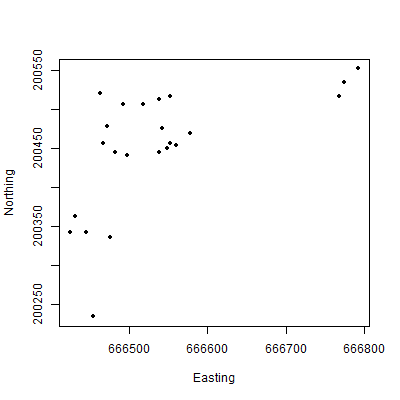
\includegraphics[height=4in,width=4in]{traps.png}
\caption{
Artificial cover object array from the slow worm study of Meier
2012).  Sampling from this array over 59 days produced encounter
histories of 44 individuals. 
}
\label{fig.fig1}
\end{figure}
An immediately obvious 'feature' of this ACO array is the irregular
and uneven distribution of cover objects.  While we may apply
capture-recapture models to the data from this study to estimate
population size $N$, it is clear that the irregular ACO array should
be a hinderance to a clear interpretation of this estimate because
there is no obvious way to compute a sample area for this
grid. Moreover, the spatial heterogeneity in trap density is almost
certain to induce heterogeneity in detection probability of
individuals depending on the location of individuals relative to
traps. While we can use model $M_h$ to account for some heterogeneity,
that model is not an explicit model of heterogeneity due to spatial
proximity of individuals to traps. Nevertheless, we fit both models
$M_0$ and $M_h$ to these data in order to see how they compare.  We
will also fit the SCR model to see how we can convert an estimate of
$N$ to density. 

We fit the logit-normal variety of model $M_h$ (Coull and Agresti
1999, Dorazio and Royle 2003) which assumes that the
logit-transformation of individual detection probabilitie $p_i$ has a
normal distribution with variance $\theta^2$:
\[
 logit(p_i) \sim \mbox{Normal}(\mu, \theta^2).
\]
Therefore this model has 3 parameters ($N$, $\mu$ and $\theta$).  The
additional parameter $\theta$ accommodates over-dispersion or
individual heterogeneity in $p$. 
For the analysis of the SCR model we defined
 the state-space by creating the minimum area rectangle around the trap array
and then buffering that by 40 meters, creating a state-space having an
area of 10.64 ha. 
The summary results from fitting these 3 models to the slow worm data
are given in Table XXXX. We note that 
AIC not comparable between SCR and ordinary closed models because the
models are fitted to different data sets:
SCR models use the individual, trap and occasion-specific
encounter data whereas ordinary capture-recapture models aggregate
over all traps to produce a simpler reduced-information individual by
occasion-specific encounter history


\begin{table}[ht]
\centering
\caption{The results of fitting models M0 and Mh and an ordinary SCR
  model to the slow worm data. }
\begin{tabular}{ccccccc}
Model &  $logit(p_0)$ &  log(n0) & extra param &   N    &  D(/ha)  &    AIC \\ \hline
 M0   & -3.189       & 3.965     &           & 47.965 &       & -73.42 \\
 Mh   & -4.193       & 3.4291899 &0.108     & 74.852 &       & -89.21 \\
SCR   &  0.050        &          & 21.02     & 154.87 & 14.56 &  320.27 \\
\end{tabular}
\end{table}





\section{Summary}

Capture-recapture methods have been the standard for estimating
population size and density for many decades. 
Capture-recapture is inherently spatial, and yet traditionally this
has almost never been addressed in the application of capture-recapture methods
 Yet these methods have
a number of deficiencies that would appear to limit their usefulness
in practice (but, strangely, have not). For example, they do not allow
the direct estimation of density, they do not account for the spatial
organization of trapping arrays, or of individuals within the
population being studied. 

The other thing is this: capture-recapture studies often involve
explicit questions about spatial ecology of species and yet
historically capture-recapture was a class of models for a systems
that is the equivalent of a vaccuum. It doesn't accommodate any kind
of interesting spatial structure.

SCR is the future........

There are several other topics related to estimation of population
size which are slightly beyond the scope of our effort here. One very
important topic is distance sampling (Buckland et al. 2001).... Unlike
capture-recapture sampling, distance sampling requires only a single
``snap-shot'' sample of the population. For each detected individual
distsance from the observer is measured.
Information about detection
probability comes from an assumed model for the relationship between
detection probability and distance to observer. 

a large body
of extensions to include open populations and other 


\section*{Literature Cited} 
\newcommand{\rf}{\vskip .1in\par\sloppy\hangindent=1pc\hangafter=1     
             \noindent}


Gibbons et al. 2000, Reading et
al. 2010) 
(B{\"o}hm et a.l 2013). 

Williams et al. 2001

\rf Royle et al. {\it in review}).  movement paper

\rf Meier 2012 thesis

\rf Alho, J. M. (1990). Logistic regression in capture-recapture models. Biometrics, 623-635.

\rf Borchers, D.L. and M.G. Efford. 2008.
Spatially explicit maximum likelihood methods for capture-recapture studies.
{\it Biometrics} 64, 377-385.

\rf Borchers, D. L., , Buckland, S. T.  and W Zucchini. 2002. Estimating animal
abundance: closed populations (Vol. 13). Springer Science \& Business Media.

\rf Boulanger, J., \& McLellan, B. (2001). Closure violation in DNA-based mark-recapture estimation of grizzly bear populations. Canadian Journal of Zoology, 79(4), 642-651.

\rf Buckland et al. 2001

\rf Christy, Michelle T., Amy A. Yackel Adams, Gordon H. Rodda, Julie
A. Savidge, and Claudine L. Tyrrell. "Modelling detection
probabilities to evaluate management and control tools for an invasive
species." Journal of Applied Ecology 47, no. 1 (2010): 106-113.


\rf Coull and Agresti 1999).
Coull, B. A., & Agresti, A. (1999). The Use of Mixed Logit Models to
Reflect Heterogeneity in Capture‐Recapture Studies. Biometrics, 55(1),
294-301.

\rf 
Converse, S. J., & Royle, J. A. (2012). Dealing with incomplete and
variable detectability in multi-year, multi-site monitoring of
ecological populations. Design and Analysis of Long-term Ecological
Monitoring Studies. Cambridge University Press, Cambridge, UK,
426-442.

\rf Dorazio, R. M., \& Andrew Royle, J. (2003). Mixture models for
estimating the size of a closed population when capture rates vary
among individuals. Biometrics, 59(2), 351-364.

\rf Dorazio, R. M., Jelks, H. L., \& Jordan, F. (2005). Improving
Removal‐Based Estimates of Abundance by Sampling a Population of
Spatially Distinct Subpopulations. Biometrics, 61(4), 1093-1101.

\rf Efford, M. 2004. Density estimation in live-trapping studies. 
{\it Oikos}  106, 598-610.

\rf Ergon, T., \& Gardner, B. (2014). Separating mortality and emigration: modelling space use, dispersal and survival with robust‐design spatial capture–recapture data. Methods in Ecology and Evolution, 5(12), 1327-1336.


\rf Huggins (1989) 
Huggins, R. M. (1989). On the statistical analysis of capture
experiments. Biometrika, 76(1), 133-140.

\rf  Karanth and Nichols 1998
Karanth, K. U., & Nichols, J. D. (1998). Estimation of tiger densities in India using photographic captures and recaptures. Ecology, 79(8), 2852-2862.

\rf Kery and Schaub (2012)
Kéry, M., & Schaub, M. (2012). Bayesian population analysis using WinBUGS: a hierarchical perspective. Academic Press.

\rf Langtimm, C. A., Dorazio, R. M., Stith, B. M., & Doyle,
T. J. (2011). New aerial survey and hierarchical model to estimate
manatee abundance. The Journal of Wildlife Management, 75(2), 399-412.

\rf Mazerolle, M. J., Bailey, L. L., Kendall, W. L., Andrew Royle, J., Converse, S. J., \& Nichols, J. D. (2007). Making great leaps forward: accounting for detectability in herpetological field studies. Journal of Herpetology, 41(4), 672-689.

\rf Norris III, J. L., \& Pollock, K. H. (1996). Nonparametric MLE under
two closed capture-recapture models with heterogeneity. Biometrics,
639-649.


\rf Otis, D. L., Burnham, K. P., White, G. C., \& Anderson,
D. R. (1978). Statistical inference from capture data on closed animal
populations. Wildlife monographs, 3-135.

\rf 
Pledger, S. (2000). Unified maximum likelihood estimates for closed
capture–recapture models using mixtures. Biometrics, 56(2), 434-442.

\rf R Development Core Team. 2004.
R: A language and environment for statistical computing.
R Foundation for Statistical Computing Vienna, Austria.


\rf Royle, J. A. (2004). Generalized estimators of avian abundance from count survey data. Animal Biodiversity and Conservation, 27(1), 375-386.



\rf Royle, J. A., R. B. Chandler, C. C. Sun, and
A. K. Fuller. 2013. Integrating resource selection information with
spatial capture-recapture. {\it Methods in Ecology and Evolution} 4(6), 520-530. 

\rf Royle, J. A., R. B. Chandler, R. Sollmann and B. 
Gardner. 2014. 
 Spatial Capture-Recapture. Academic Press.

\rf Royle, J. A. 2009. Analysis of capture-recapture models with
individual covariates using data augmentation. {\it Biometrics} 
  65(1), 267-274.

\rf Royle, J.A., R.M. Dorazio and W.A. Link. 2007. Analysis of multinomial 
models with unknown index using data augmentation. 
{\it Journal of Computational and Graphical Statistics}  16, 67-85.

\rf Royle, J. A. and R. M. Dorazio. 2012. Parameter-expanded data
augmentation for Bayesian analysis of capture-recapture
models. {\it Journal of Ornithology} 152(2), 521-537.

\rf  Royle, J.A. and K.V. Young. 2008. 
A hierarchical model for spatial capture-recapture data.
{\it Ecology}  89, 2281-2289.

\rf Royle, J. A., Chandler, R. B., Gazenski, K. D., \& Graves,
T. A. (2013). Spatial capture-recapture models for jointly estimating
population density and landscape connectivity. Ecology, 94(2),
287-294.

\rf Royle, J. A., Converse, S. J., \& Link, W. A. (2012). Data Augmentation
for Hierarchical Capture-recapture Models. arXiv preprint
arXiv:1211.5706.


\rf Schaub, M., \& Royle, J. A. (2014). Estimating true instead of apparent
survival using spatial Cormack–Jolly–Seber models. Methods in Ecology
and Evolution, 5(12), 1316-1326.


\rf Sutherland, C., A. K. Fuller and J. A. Royle. 2015. Modelling
non-Euclidean movement and landscape connectivity in highly structured
ecological networks. {\it Methods in Ecology and Evolution}  6, 169-177.

\rf Tanner, M. A., \& Wong, W. H. (1987). The calculation of posterior
distributions by data augmentation. Journal of the American
statistical Association, 82(398), 528-540.

\rf Tyrrell, Claudine L., Michelle T. Christy, Gordon H. Rodda, Amy
A. Yackel Adams, Aaron R. Ellingson, Julie A. Savidge, Kathy
Dean-Bradley, and Richard Bischof. "Evaluation of trap capture in a
geographically closed population of brown treesnakes on Guam." Journal
of Applied Ecology 46, no. 1 (2009): 128-135.


\rf Yang, H. C., \& Chao, A. (2005). Modeling animals' behavioral response
by Markov chain models for capture–recapture experiments. Biometrics,
61(4), 1010-1017.

\rf Zylstra, Erin R., Robert J. Steidl, and Don E. Swann. "Evaluating
survey methods for monitoring a rare vertebrate, the Sonoran desert
tortoise." The Journal of Wildlife Management 74.6 (2010): 1311-1318.

\end{document}


